\RequirePackage{ifpdf}
\ifpdf
	\documentclass[11pt,oneside,a4paper,pdftex]{article}   %two-page printing
\else
	\documentclass[11pt,twoside,a4paper,dvips]{article}   %two-page printing
\fi

%\documentclass[a4paper, 12pt]{article}
\addtolength{\hoffset}{-1.9cm}
\addtolength{\voffset}{-1.9cm}
\addtolength{\textwidth}{+3.8cm}
\addtolength{\textheight}{+3.8cm}
\usepackage[latin1,utf8]{inputenc}
\usepackage[czech]{babel}
\usepackage{icomma} % ceska desetinna carka
\usepackage{csquotes}
\usepackage{listings}
\usepackage{amsmath}
\usepackage{amsthm}
\usepackage{amsfonts}
\usepackage{mathrsfs}
%\usepackage[T1]{fontenc}
\ifpdf
	\usepackage[pdftex]{graphicx} % dvips or pdftex
\else
	\usepackage[dvips]{graphicx} % dvips or pdftex
\fi
\usepackage[center]{subfigure}
\usepackage{amsfonts}
\usepackage[dvips]{color}               %for using colors
%\usepackage{showframe}                 %zobrazuje okraje stranky
\usepackage[justification=justified,hang]{caption}
\usepackage{textpos}
\usepackage{url}
%\usepackage{fancybox}
\usepackage{verbatim}
\usepackage{fj}
\ifpdf
	\usepackage[pdftex,unicode,colorlinks]{hyperref}
\else
	\usepackage[unicode]{hyperref}
\fi


\title{A4M33TDV Homework H4: "Binary partitionings and maximal matchings" (p. 176)}
\date{1. 1. 2012}
\author{Filip Jareš}

\begin{document}
\selectlanguage{english}

\maketitle

\section{Assignment}

Let $T$ be a $N\times N$ matching table.  How many are there:
\begin{enumerate}
	\item[(1)] binary partitionings of $T$,
	\item[(2)] maximal matchings in $T$;
\end{enumerate}
prove the results.

% \begin{figure}[htb]
% 	\centering
% 	\subfigure[] {
% 		\fbox{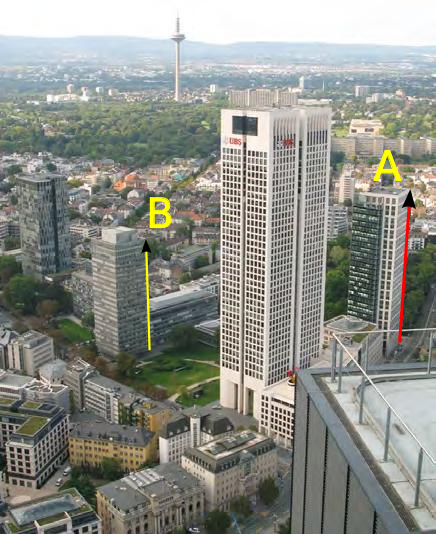
\includegraphics[width=6.5cm]{buildings-with_arrows.jpeg}}
% 		\label{photo}
% 	}
% 	\subfigure[] {
% 		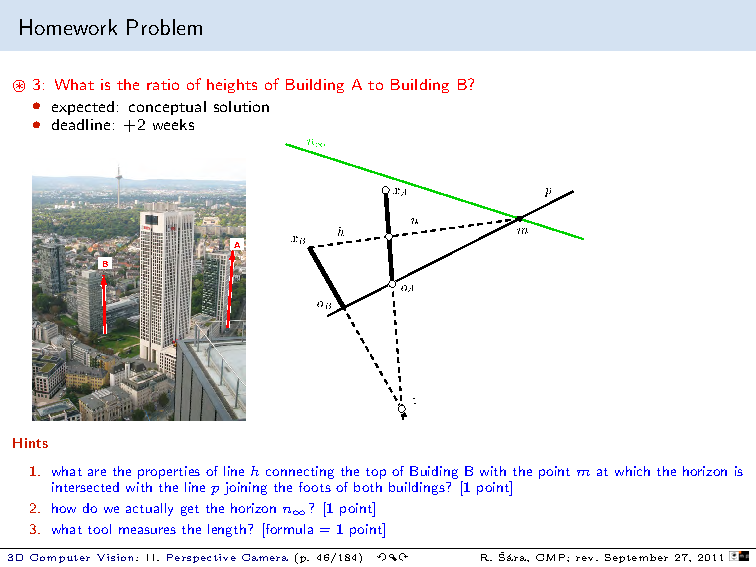
\includegraphics[width=6.5cm,clip=true,trim=4.5cm 2cm 3cm 2cm]{pg_0019.pdf}
% 		\label{scheme}
% 	}
% 	\caption{}
% 	\label{buildings}
% \end{figure}

\section{Solution}

\paragraph{Solution to (1)}

For $N \times N$ matching table there are $2^{N^2}$ binary partitionings.

\paragraph{Solution to (2)}

According to \cite[p. 168]{SaraLectures} a set of pairs $M = \{p_i\}_{i=1}^n$,
$p_i \in T$ is a matching if and only if it satisfies the uniqueness constraint
\eqref{eq:uniqueness}.
	\begin{equation}
		\label{eq:uniqueness}
		\forall p_i, p_j \in M, i \ne j: p_j \notin X(p_i).
	\end{equation}
Here $X(p_i)$ denotes set of pairs in matching table that are ruled out by the
pair $p_i$. For a pair $p = (i, j)$ the set $X(p)$ is formed by union of all
pairs $q$ which are different from $p$ and which lie in the same row or in
the same column in the matching table as $p$:
	\begin{equation}
		X(p)	= X((i, j))
			= \{ q = (k,l) \in T \ |\ 
			  (k = i \vee l = j) \wedge q \ne p \}.
	\end{equation}
Maximal matchings for square matching tables are such that they have (exactly
one) pair in each row and each column of the matching table. Therefore the count
of maximal matchings in a $N \times N$ matching table is equal to count of
permutations of set of $N$ elements. That is count of maximal matchings is $N!$.

% \section{Optional task}
% 
% \paragraph{Assignment} How many are there maximal monotonic matchings?
% 
% \paragraph{Solution}


\bibliographystyle{czechiso}
\bibliography{bibliography}

\end{document}

